\documentclass[a4paper,12pt,oneside,onecolumn]{book}
\linespread{1.5}
\usepackage[utf8]{inputenc}                                      
\usepackage[T1]{fontenc}  
\usepackage{helvet}
\renewcommand{\familydefault}{\sfdefault}
\usepackage{amsmath,amsfonts,amssymb,amsthm}
\usepackage[british,polish]{babel}
\usepackage{csquotes}
\usepackage[margin=2.5cm]{geometry}
\usepackage{graphicx}
\usepackage{xcolor}
\usepackage{array}
\graphicspath{ {images/} } % folder z grafiką
\usepackage{url}
\usepackage{hyperref}
\usepackage{indentfirst}
\usepackage{microtype}
\tolerance=1000
\emergencystretch=3em
\hfuzz=2pt
\usepackage[natbib=true,backend=biber,maxbibnames=99,defernumbers=true]{biblatex}
\usepackage{listings}
\usepackage{fancyhdr}
\usepackage{etoolbox}
\patchcmd{\chapter}{\thispagestyle{plain}}{\thispagestyle{fancy}}{}{}

% % *** Listings Style ***
\definecolor{codegreen}{rgb}{0,0.6,0}
\definecolor{codegray}{rgb}{0.5,0.5,0.5}
\definecolor{codepurple}{rgb}{0.58,0,0.82}
\definecolor{backcolour}{rgb}{0.95,0.95,0.92}

\lstdefinestyle{mystyle}{
    backgroundcolor=\color{backcolour},   
    commentstyle=\color{codegreen},
    keywordstyle=\color{magenta},
    numberstyle=\tiny\color{codegray},
    stringstyle=\color{codepurple},
    basicstyle=\ttfamily\footnotesize,
    breakatwhitespace=false,         
    breaklines=true,                 
    captionpos=b,                    
    keepspaces=true,                 
    numbers=left,                    
    numbersep=5pt,                  
    showspaces=false,                
    showstringspaces=false,
    showtabs=false,                  
    tabsize=2
}

\lstset{style=mystyle}

\renewcommand{\lstlistingname}{Próbka kodu}
\renewcommand{\lstlistlistingname}{Spis próbek kodu}
\renewcommand{\listfigurename}{Spis rysunków}
\renewcommand{\listtablename}{Spis tabel}
\renewcommand{\figurename}{Rysunek}
\renewcommand{\tablename}{Tabela}

\newenvironment{conditions}
  {\par\vspace{\abovedisplayskip}\noindent\begin{tabular}{>{$}l<{$} @{${}={}$} l}}
  {\end{tabular}\par\vspace{\belowdisplayskip}}


\addbibresource{refs.bib}
\addbibresource{url_refs.bib}

\begin{document}

% *************** Front matter ***************
% *************** Strona tytułowa ***************

\newcommand{\thesistitlepl}{Model predykcji formy kolarskiej oparty na danych telemetrycznych z urządzeń sportowych z wykorzystaniem uczenia maszynowego}
\newcommand{\thesistitleen}{A Machine Learning-Based Model for Predicting Cycling Performance Using Telemetry Data from Sports Devices}
\newcommand{\thesisauthor}{Rafał Banaś}
\newcommand{\thesisfield}{Informatyka}
\newcommand{\thesisalbum}{152863}
\newcommand{\thesispromoter}{dr Barbary Probierz}

\pagestyle{empty}
\begin{center}
\vspace*{1.25cm}
UNIWERSYTET EKONOMICZNY W KATOWICACH

\vspace{0.65cm}
\MakeUppercase{\thesisfield}

\vspace{2.25cm}
{\bfseries \MakeUppercase{\thesisauthor}}\\
{\bfseries \thesisalbum}

\vspace{3.25cm}
{\bfseries\fontsize{18}{22}\selectfont \MakeUppercase{\thesistitlepl}\par}

\vspace{0.65cm}
{\bfseries\fontsize{13}{16}\selectfont \MakeUppercase{\thesistitleen}\par}
\end{center}

\vfill
\hfill
\begin{minipage}{0.58\textwidth}
\raggedright
Praca magisterska napisana\\
pod kierunkiem \thesispromoter
\end{minipage}

\vspace{2.3cm}
\begin{center}
KATOWICE 2026
\end{center}

\newpage 

\pagestyle{fancy}
\fancyhf{}
\renewcommand{\headrulewidth}{0pt}
\fancyfoot[R]{\thepage}

\vspace*{0.6cm}
\begin{center}
    \textbf{OŚWIADCZENIE PROMOTORA}
\end{center}

\vspace{0.45cm}
\noindent Oświadczam, że niniejsza praca została przygotowana pod moim kierunkiem i stwierdzam,
że spełnia wymogi stawiane pracom dyplomowym.

\vspace{0.45cm}
\noindent Pracę akceptuję

\vspace{0.85cm}
\begin{minipage}{2in}
\begin{center}
\dotfill \\
(data)
\end{center}
\end{minipage}
\hfill
\begin{minipage}{2in}
\begin{center}
\dotfill \\
(podpis promotora)
\end{center}
\end{minipage}

\newpage

% *************** Oświadczenie początkowe ***************
\begingroup
\fontsize{11}{14}\selectfont
\vspace*{0.1cm}
\noindent
\begin{minipage}[t]{0.42\textwidth}
\begin{center}
\makebox[\linewidth]{\thesisauthor}\\[-0.15cm]
\dotfill\\[-0.2cm]
Imię i nazwisko

\vspace{0.2cm}
\makebox[\linewidth]{\thesisfield}\\[-0.15cm]
\dotfill\\[-0.2cm]
Kierunek

\vspace{0.2cm}
\makebox[\linewidth]{\thesisalbum}\\[-0.15cm]
\dotfill\\[-0.2cm]
Nr albumu
\end{center}
\end{minipage}
\hfill
\begin{minipage}[t]{0.52\textwidth}
 \begin{flushright}
Katowice, dnia \dotfill
 \end{flushright}
\end{minipage}

\vspace{0.25cm}
\begin{center}
    \textbf{OŚWIADCZENIE}
\end{center}

\vspace{0.1cm}
\noindent Mając świadomość odpowiedzialności prawnej oświadczam, że złożona praca magisterska pt.

\vspace{0.1cm}
\noindent\dotfill

\noindent\thesistitlepl

\noindent\dotfill

\noindent została napisana przeze mnie samodzielnie.
Równocześnie oświadczam, że praca ta nie narusza praw autorskich w rozumieniu ustawy z dnia 4 lutego 1994 roku o prawie autorskim i prawach pokrewnych oraz dóbr osobistych chronionych prawem.
Ponadto praca nie zawiera informacji i danych uzyskanych w sposób niedozwolony i nie była wcześniej przedmiotem innych procedur związanych z uzyskaniem dyplomów lub tytułów zawodowych uczelni wyższej.
Wyrażam zgodę na nieodpłatne udostępnienie mojej pracy w celu oceny jej oryginalności przez Jednolity System Antyplagiatowy prowadzony przez ministra właściwego ds. szkolnictwa wyższego oraz przechowywania jej w Ogólnopolskim Repozytorium Prac Dyplomowych oraz wewnętrznej bazie prac dyplomowych Uniwersytetu Ekonomicznego w Katowicach. Oświadczam, że poinformowano mnie o zasadach dotyczących oceny oryginalności pracy dyplomowej przez Jednolity System Antyplagiatowy.
Oświadczam także, że ostateczna wersja pracy przesłana przeze mnie drogą elektroniczną jest zgodna z plikiem poddanym ocenie w Jednolitym Systemie Antyplagiatowym.
Jednocześnie oświadczam, że jest mi znany przepis art. 233 § 1 Kodeksu karnego określający odpowiedzialność za składanie fałszywych zeznań.

\begin{flushright}
\makebox[0.52\textwidth]{\dotfill} \\
(podpis składającego oświadczenie)
\end{flushright}
\endgroup


% *************** Spis treści ***************
\tableofcontents

% *************** Koniec front matter ***************


\chapter{Wprowadzenie w tematykę pracy}

W ostatnich latach rozwój sensorów i urządzeń treningowych umożliwił sportowcom amatorskim i zawodowym gromadzenie dużych ilości danych telemetrycznych opisujących przebieg aktywności fizycznej. W kolarstwie do najważniejszych zmiennych należą moc generowana przez zawodnika oraz tętno, kadencja i prędkość. Analiza takich danych otwiera nowe możliwości zarówno w zakresie monitorowania obciążeń treningowych, jak i w przewidywaniu poziomu formy sportowej.

Celem niniejszej pracy jest opracowanie modelu predykcyjnego pozwalającego na szacowanie funkcjonalnego progu mocy (Functional Threshold Power, FTP) na podstawie szeregów czasowych rejestrowanych podczas jazdy na rowerze. FTP jest parametrem szeroko stosowanym przez kolarzy do planowania treningów i oceny wydolności, jednak jego tradycyjne wyznaczenie wymaga specjalistycznych testów terenowych lub laboratoryjnych. Proponowane rozwiązanie oparte na uczeniu maszynowym ma na celu umożliwienie estymacji tego parametru bez potrzeby wykonywania dedykowanego testu, a jedynie w oparciu o dane zebrane podczas zwykłych sesji treningowych.

Zakres pracy obejmuje analizę literatury dotyczącej pomiaru i interpretacji FTP, charakterystykę dostępnych źródeł danych telemetrycznych oraz opis metodyki ich przetwarzania. W kolejnych rozdziałach przedstawione zostaną etapy przygotowania zbioru danych, inżynierii cech, budowy modeli regresyjnych oraz oceny ich skuteczności na podstawie wybranych metryk.

Praca kończy się dyskusją uzyskanych wyników, wskazaniem ograniczeń zaproponowanego podejścia oraz propozycjami dalszego rozwoju w kierunku bardziej precyzyjnych i adaptacyjnych algorytmów predykcyjnych.




\chapter{Podstawy teoretyczne estymacji parametrów wydolnościowych z wykorzystaniem uczenia maszynowego}

Wydolność tlenowa w kolarstwie jest jednym z kluczowych czynników determinujących wynik sportowy \cite{borszcz2018ftp}.
Jej ilościowy opis od lat stanowi przedmiot badań fizjologów wysiłku i trenerów.
W praktyce treningowej potrzebne są wskaźniki, które z jednej strony dobrze odzwierciedlają możliwości zawodnika, a z drugiej są możliwe do regularnego monitorowania w warunkach terenowych.
Jednym z najczęściej stosowanych parametrów jest funkcjonalny próg mocy (ang. \textit{Functional Threshold Power}, $\mathrm{FTP}$) \cite{borszcz2018ftp,allen2019power}.

Rozwój czujników pomiaru mocy, opasek rejestrujących tętno oraz szerokie wykorzystanie liczników rowerowych i platform treningowych powoduje, że powstają liczne zbiory danych treningowych.
Dane te mogą zostać wykorzystane w modelach uczenia maszynowego do estymacji $\mathrm{FTP}$ na podstawie codziennych jazd, bez potrzeby wykonywania osobnych, wyczerpujących testów.

W niniejszym rozdziale przedstawiono podstawowe pojęcia związane z $\mathrm{FTP}$, charakterystykę danych wykorzystywanych w dalszej części pracy oraz przegląd wybranych metod szacowania parametrów wydolnościowych z użyciem klasycznych podejść i uczenia maszynowego.

\section{FTP jako parametr wydolności}

Funkcjonalny próg mocy ($\mathrm{FTP}$) jest jednym z najczęściej stosowanych w praktyce treningowej wskaźników wydolności tlenowej kolarzy \cite{borszcz2018ftp,allen2019power}.
Intuicyjnie można go opisać jako „moc, którą kolarz jest w stanie utrzymać przez dłuższy czas bez narastającego, gwałtownego zmęczenia”.
W przeciwieństwie do prostych wartości maksymalnych (np.\ maksymalnej mocy szczytowej czy tętna maksymalnego), $\mathrm{FTP}$ odnosi się do zdolności organizmu do długotrwałego utrzymania wysokiej, ale jeszcze zrównoważonej intensywności wysiłku.
Z tego powodu parametr ten dobrze nadaje się do opisu poziomu sportowego i planowania treningu wytrzymałościowego.

\subsection{Definicja funkcjonalnego progu mocy}

W literaturze związanej z treningiem kolarskim parametr $\mathrm{FTP}$ najczęściej definiuje się jako najwyższą wartość mocy, jaką kolarz jest w stanie utrzymać w stanie quasi-stacjonarnym przez około $60$ minut \cite{borszcz2018ftp,allen2019power}.
„Quasi-stacjonarny” oznacza tutaj, że reakcja fizjologiczna organizmu (w szczególności tętno, wentylacja oraz stężenie mleczanu we krwi) stabilizują się na podwyższonym, ale względnie stałym poziomie.
W praktyce przyjmuje się, że przy mocy równej $\mathrm{FTP}$ parametry te nie narastają już gwałtownie, natomiast przekroczenie tej intensywności prowadzi do szybkiego narastania zmęczenia i konieczności zredukowania mocy \cite{borszcz2018ftp,karsten2021cpftp}.

Ze względów praktycznych $\mathrm{FTP}$ rzadko wyznacza się z pełnego, $60$-minutowego testu czasowego.
Taki test jest bardzo obciążający, wymaga odpowiednich warunków i trudno go często powtarzać.
Dlatego w treningu amatorskim i zawodowym spopularyzowały się krótsze protokoły, z których najpopularniejszy jest $20$-minutowy test maksymalny \cite{allen2019power}.
Uproszczona wersja polega na wykonaniu rozgrzewki, a następnie jeździe z maksymalnym możliwym wysiłkiem  przez $20$ minut.
Średnia moc z tego odcinka jest następnie mnożona przez współczynnik (najczęściej $0{,}95$), co ma przybliżać moc, jaką kolarz byłby w stanie utrzymać przez $60$ minut \cite{allen2019power,sitko2023update}.

\begin{equation}
\label{eq:ftp_20min}
\mathrm{FTP} \approx 0{,}95 \cdot \overline{P}_{20\ \mathrm{min}},
\end{equation}
gdzie $\overline{P}_{20\ \mathrm{min}}$ oznacza średnią moc w $20$-minutowym odcinku testowym.

Warto podkreślić, że jest to definicja funkcjonalna, a nie „fizjologiczna” w ścisłym sensie.
$\mathrm{FTP}$ nie jest bezpośrednim pomiarem żadnego pojedynczego mechanizmu w organizmie (np.\ maksymalnego poboru tlenu), lecz wygodnym parametrem łączącym w sobie kilka aspektów wydolności: zdolność do generowania mocy, tolerancję zmęczenia i efektywność procesów metabolicznych \cite{borszcz2018ftp,karsten2021cpftp}.

\subsection{Znaczenie pomiaru mocy w treningu kolarskim}

Współczesny trening kolarski coraz częściej opiera się na pomiarze mocy generowanej przez zawodnika.
W przeciwieństwie do tętna czy subiektywnego odczucia wysiłku (ang.\ \textit{Rate of Perceived Exertion}, $\mathrm{RPE}$), moc jest parametrem bezpośrednio opisującym pracę mechaniczną wykonywaną na rowerze.
Informuje wprost, ile energii w jednostce czasu kolarz przekazuje na napędzanie roweru, niezależnie od takich czynników jak stres, temperatura otoczenia czy chwilowe wahania nastroju \cite{allen2019power,phases2023ftp}.

Pomiar mocy ma kilka kluczowych zalet z punktu widzenia planowania i analizy treningu:
\begin{itemize}
  \item \textbf{Obiektywność i powtarzalność} - ta sama wartość mocy oznacza ten sam poziom obciążenia zewnętrznego, niezależnie od dnia i samopoczucia zawodnika. Ułatwia to porównywanie wysiłków w czasie oraz między różnymi jednostkami treningowymi.
  \item \textbf{Dokładne sterowanie intensywnością} - strefy treningowe oparte na procentach $\mathrm{FTP}$ pozwalają precyzyjnie dozować obciążenie (np.\ trening progowy, $\text{VO}_{2\max}$, jazdy regeneracyjne), co sprzyja świadomemu kształtowaniu określonych adaptacji fizjologicznych \cite{allen2019power}.
  \item \textbf{Lepsza analiza obciążeń niż na podstawie tętna} - tętno reaguje z opóźnieniem i podlega wpływowi temperatury, odwodnienia czy stresu. Moc zmienia się natychmiast po zmianie nacisku na pedały, dzięki czemu lepiej odzwierciedla przebieg wysiłku.
  \item \textbf{Możliwość zaawansowanej analizy danych} - rejestracja mocy w czasie pozwala obliczać wskaźniki (np.\ moc znormalizowana $\mathrm{NP}$, $\mathrm{TSS}$, czas spędzony w strefach), a także stosować modele matematyczne i metody uczenia maszynowego \cite{stockwell2023mlftp,denham2020predictftp}.
  \item \textbf{Monitorowanie postępu i zmęczenia} - analiza danych z codziennych treningów umożliwia szacowanie zmian $\mathrm{FTP}$ i ogólnego poziomu wytrenowania bez konieczności częstego wykonywania formalnych testów laboratoryjnych \cite{borszcz2018ftp,karsten2021cpftp,denham2020predictftp}.
\end{itemize}

Z tych powodów moc stała się jednym z podstawowych parametrów używanych w treningu kolarskim na każdym poziomie zaawansowania - od amatorów po zawodowców.
W kontekście niniejszej pracy jest to szczególnie istotne, ponieważ $\mathrm{FTP}$ pełni rolę kluczowego wskaźnika wydolności opartego właśnie na danych z pomiaru mocy.

\subsection{Znaczenie FTP w praktyce treningowej}

$\mathrm{FTP}$ jest szeroko stosowane zarówno w badaniach naukowych, jak i w codziennej praktyce trenerów i kolarzy \cite{borszcz2018ftp,allen2019power,karsten2021cpftp,denham2020predictftp}.
Wartość tego parametru służy przede wszystkim do:
\begin{itemize}
  \item wyznaczania stref treningowych - zakresy mocy (lub tętna) definiuje się jako procent $\mathrm{FTP}$, co pozwala opisywać intensywność treningu w sposób bardziej obiektywny niż wyłącznie na podstawie odczuć;
  \item monitorowania postępów - wzrost $\mathrm{FTP}$ (np.\ z $250\ \mathrm{W}$ do $270\ \mathrm{W}$) w pewnym okresie czasu interpretuje się jako poprawę wydolności tlenowej;
  \item porównywania zawodników - przeliczenie $\mathrm{FTP}$ na wartość względną $\mathrm{W\,kg^{-1}}$ pozwala porównywać kolarzy o różnej masie ciała;
  \item planowania strategii wyścigowych - znajomość $\mathrm{FTP}$ pomaga oszacować tempo możliwe do utrzymania na długich podjazdach czy w jeździe indywidualnej na czas.
\end{itemize}

Z punktu widzenia uczenia maszynowego $\mathrm{FTP}$ jest naturalnym kandydatem na zmienną wyjściową (etykietę, $y$) w modelach regresyjnych.
Oznacza to, że model ma za zadanie przybliżyć zależność pomiędzy zarejestrowanymi danymi z treningów (moc, tętno, czas, parametry trasy) a „ukrytą” wartością $\mathrm{FTP}$ danego zawodnika \cite{stockwell2023mlftp,denham2020predictftp}.

\subsection{Podstawy fizjologii wysiłku istotne dla interpretacji FTP}

Aby poprawnie interpretować dane używane przez model oraz ograniczenia tradycyjnych testów $\mathrm{FTP}$, wystarczy uproszczony obraz fizjologii wysiłku:
\begin{itemize}
  \item \textbf{Układ krążenia i tlen.} W trakcie wysiłku mięśnie potrzebują tlenu do wytwarzania energii. Serce pompuje krew bogatą w tlen, a tętno rośnie wraz z intensywnością wysiłku. W średnich intensywnościach wzrost mocy często wiąże się z niemal liniowym wzrostem tętna.
  \item \textbf{Progi metaboliczne.} Przy coraz większej intensywności organizm w coraz większym stopniu korzysta z procesów beztlenowych, a we krwi kumuluje się mleczan. W okolicach progów mleczanowych lub wentylacyjnych równowaga pomiędzy produkcją a usuwaniem mleczanu jest na granicy: organizm jest jeszcze w stanie utrzymać wysiłek, ale przy dalszym zwiększaniu obciążenia równowaga się załamuje i dochodzi do szybkiego narastania zmęczenia. $\mathrm{FTP}$ jest zwykle zlokalizowane w pobliżu tych progów, ale nie jest z nimi tożsame \cite{borszcz2018ftp,karsten2021cpftp,denham2020predictftp}.
  \item \textbf{Dryf tętna (ang.\ \textit{cardiac drift}).} Podczas dłuższych wysiłków przy stałej mocy często obserwuje się zjawisko stopniowego wzrostu tętna w czasie, mimo że moc nie rośnie. Wynika to m.in.\ z narastającego zmęczenia, zmian w termoregulacji i niewielkiego spadku objętości krwi krążącej. Oznacza to, że relacja „moc--tętno” nie jest idealnie stała: ta sama moc po $5$ minutach i po $40$ minutach może odpowiadać innemu tętnu. Ponadto tętno reaguje na zmiany mocy z opóźnieniem (tzw.\ \textit{HR lag}), więc po nagłym zwiększeniu lub zmniejszeniu obciążenia serce potrzebuje zwykle kilkudziesięciu sekund, aby „dogonić” nowy poziom wysiłku. Z punktu widzenia modeli uczonych na danych sekunda-po-sekundzie oznacza to, że bieżąca wartość tętna odzwierciedla raczej średnie obciążenie z ostatnich kilkudziesięciu sekund niż chwilowy odczyt mocy.
\end{itemize}

\begin{figure}[htbp]
  \centering
  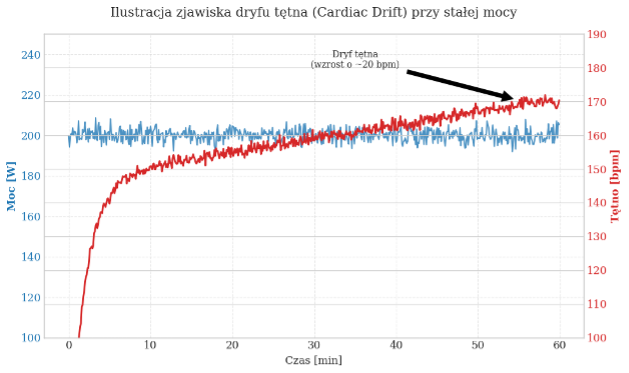
\includegraphics[width=0.95\linewidth]{figures/fig1_hr_drift_hr_lag.png}
  \caption{Ilustracja zjawiska dryfu tętna przy stałej mocy oraz widoczne opóźnienie narastania tętna (\textit{HR lag}) w początkowej fazie wysiłku \cite{nomadfrontiers_power_hr,bikeradar_power_hr}. Źródło: Opracowanie własne.
  }
  \label{fig:hr_drift_hr_lag}
\end{figure}

Dodatkowo:
\begin{itemize}
  \item \textbf{Zmęczenie i wyczerpanie.} Gdy intensywność przekracza zdolność organizmu do stabilnego utrzymania równowagi metabolicznej, narastające zmęczenie prowadzi do konieczności zmniejszenia mocy. W testach $\mathrm{FTP}$ objawia się to przerwaniem wysiłku lub znaczącym obniżeniem mocy, co widać jako spadek mocy na wykresie \cite{borszcz2018ftp,karsten2021cpftp}.
\end{itemize}

Z perspektywy modelu uczenia maszynowego oznacza to, że:
\begin{itemize}
  \item sygnał tętna zawiera informację o reakcji organizmu na obciążenie (moc),
  \item relacja moc--tętno jest nieliniowa i zmienia się w czasie (dryf, narastające zmęczenie),
  \item pojedynczy test $\mathrm{FTP}$ jest jedynie pojedynczym pomiarem tej relacji w konkretnych warunkach oraz w konkretnym dniu.
\end{itemize}

Dlatego sensowne jest podejście, w którym model uczy się tej relacji z wielu treningów, zamiast polegać wyłącznie na jednym teście \cite{stockwell2023mlftp,denham2020predictftp}.

\subsection{Test 20-minutowy -- przebieg i ilustracja}

Najpopularniejszy protokół używany w praktyce do wyznaczania $\mathrm{FTP}$ to test $20$-minutowy \cite{allen2019power,sitko2023_ac20to60_update,phasescycling2023_ftp_variability}.
W literaturze i poradnikach trenerskich spotyka się różne wersje, ale typowy schemat wygląda następująco:
\begin{itemize}
  \item \textbf{Rozgrzewka} (ok.\ $10$--$20$ minut): jazda o niskiej i umiarkowanej intensywności, często z krótkimi przyspieszeniami.
  \item \textbf{Wysiłki przygotowujące} (ang.\ \textit{openers}): krótki, kilku-minutowy wysiłek na wysokiej intensywności (np.\ $3$--$5$ minut powyżej $\mathrm{FTP}$), a następnie etap spokojnej jazdy.
  \item \textbf{Odpoczynek / spokojna jazda} (kilka--kilkanaście minut): częściowa regeneracja przy utrzymaniu „rozgrzania”.
  \item \textbf{Część główna}: $20$-minutowy wysiłek maksymalny; zawodnik stara się utrzymać możliwie najwyższą średnią moc przez pełne $20$ minut.
\end{itemize}

\begin{figure}[htbp]
  \centering
  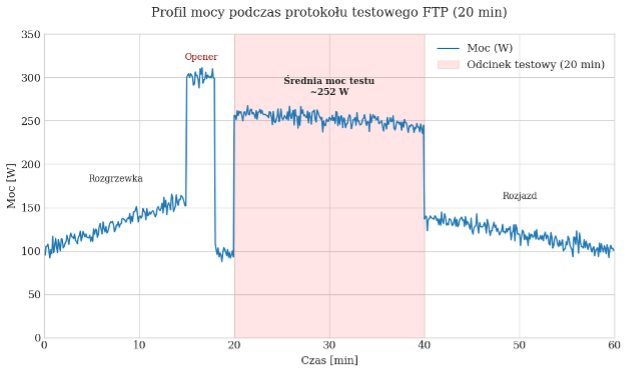
\includegraphics[width=0.95\linewidth]{figures/fig2_ftp_test_20min_schema.png}
  \caption{Schemat przebiegu testu $20$-minutowego $\mathrm{FTP}$: rozgrzewka, wysiłek przygotowujący, okres spokojnej jazdy i $20$-minutowy wysiłek maksymalny. Wynik z otrzymaną średnią należy przemnożyć przez $0{,}95$ \cite{trainerroad_ftp_tips}. Źródło: Opracowanie własne.
  }
  \label{fig:test_20min_schema}
\end{figure}

Dodatkowo można rozważyć drugi wykres, na którym przy stałej mocy podczas $20$-minutowego odcinka widoczny jest stopniowy wzrost tętna jako ilustracja zjawiska dryfu tętna omawianego w poprzedniej sekcji.

\subsection{Test 60-minutowy -- przebieg i ilustracja}

Choć w praktyce trenerskiej najczęściej stosuje się skrócone protokoły (np.\ test $20$-minutowy), pełny, $60$-minutowy test czasowy uznawany jest za najbardziej bezpośrednią i klasyczną metodę wyznaczania $\mathrm{FTP}$.
W ujęciu historycznym $\mathrm{FTP}$ definiowano jako moc, którą zawodnik jest w stanie utrzymać przez pełną godzinę jazdy ciągłej.
Wymaga to jednak bardzo wysokiej dyspozycji, odpowiedniego przygotowania mentalnego oraz sprzyjających warunków, dlatego test stosuje się głównie w środowisku laboratoryjnym lub u doświadczonych kolarzy \cite{allen2019power,sitko2023update}.

Typowy protokół $60$-minutowy można przedstawić następująco:
\begin{itemize}
  \item \textbf{Rozgrzewka} ($15$--$20$ minut): jazda o niższej i umiarkowanej intensywności z kilkoma krótkimi przyspieszeniami.
  \item \textbf{Wstępne pobudzenie} (ang.\ \textit{openers}): kilkuminutowy wysiłek na wysokiej intensywności (np.\ $2$--$4$ minuty powyżej $\mathrm{FTP}$), po którym następuje spokojniejszy fragment jazdy.
  \item \textbf{Krótki etap spokojniejszej jazdy} ($5$--$10$ minut): tętno nieco opada, zawodnik pozostaje przygotowany do części głównej.
  \item \textbf{Część główna}: $60$-minutowy wysiłek submaksymalny o możliwie stałej mocy; średnia moc z tego odcinka jest bezpośrednio interpretowana jako $\mathrm{FTP}$ (bez przelicznika).
\end{itemize}

\begin{figure}[htbp]
  \centering
  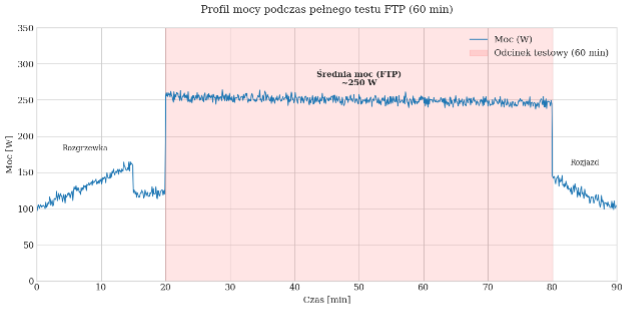
\includegraphics[width=0.95\linewidth]{figures/fig3_ftp_test_60min_schema.png}
  \caption{Schemat przebiegu pełnego testu $60$-minutowego $\mathrm{FTP}$: rozgrzewka, wysiłek przygotowujący, krótki etap spokojnej jazdy oraz główny, godzinny odcinek o możliwie stałej mocy. Średnia moc z $60$-minutowego segmentu stanowi bezpośredni wyznacznik $\mathrm{FTP}$. Źródło: Opracowanie własne.}
  \label{fig:test_60min_schema}
\end{figure}

\subsection{Krzywa mocy i zależność FTP od czasu trwania wysiłku}

Schematyczną zależność maksymalnej możliwej do utrzymania mocy od czasu trwania wysiłku przedstawiono na rysunku \ref{fig:power_duration_curve}.
Dla bardzo krótkich czasów wartości mocy są wysokie i szybko maleją, natomiast przy dłuższych wysiłkach krzywa stopniowo zbliża się do poziomu odpowiadającego mocy krytycznej (ang.\ \textit{Critical Power}, $\mathrm{CP}$), która jest blisko spokrewniona z funkcjonalnym progiem mocy ($\mathrm{FTP}$) \cite{borszcz2018ftp,allen2019power,karsten2021cpftp}.

\begin{figure}[htbp]
  \centering
  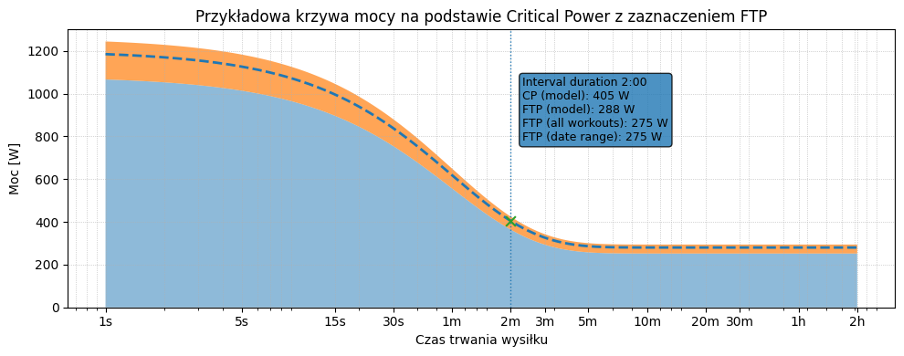
\includegraphics[width=0.95\linewidth]{figures/fig4_power_duration_curve_cp_ftp.png}
  \caption{Przykładowa krzywa mocy (\textit{power--duration}) na podstawie koncepcji mocy krytycznej, z zaznaczonym $2$-minutowym odcinkiem wysiłku i przykładowymi wartościami $\mathrm{FTP}$ (opracowanie własne na podstawie \textit{PerfectPace, The Critical Power Chart}). Źródło: Opracowanie własne.}
  \label{fig:power_duration_curve}
\end{figure}

W praktyce platformy treningowe i oprogramowanie analityczne wykorzystują takie krzywe do estymacji parametrów wydolnościowych, w tym $\mathrm{FTP}$, na podstawie danych z wielu treningów bez konieczności wykonywania osobnego testu \cite{borszcz2018ftp,allen2019power,karsten2021cpftp,denham2020predictftp}.

\section{Charakterystyka danych treningowych}

Modele uczenia maszynowego wykorzystywane do estymacji $\mathrm{FTP}$ opierają się na danych rejestrowanych podczas jazdy na rowerze.
Podstawowym źródłem informacji jest miernik mocy instalowany w korbie, piaście, pedale lub suporcie, który z wysoką częstotliwością (najczęściej $1\ \mathrm{Hz}$) rejestruje chwilową moc generowaną przez kolarza.
Równolegle rejestrowane jest tętno za pomocą opaski na klatkę piersiową lub optycznego czujnika na nadgarstku.
W zależności od konfiguracji sprzętu oraz platformy treningowej możliwe jest także zapisywanie dodatkowych parametrów, takich jak kadencja, prędkość, położenie GPS, nachylenie trasy czy wysokość nad poziomem morza \cite{allen2019power,phases2023ftp,kaggle_cycling_data,figshare_cycling_data}.

W kontekście uczenia maszynowego dane te mają postać szeregów czasowych: dla każdej sekundy otrzymujemy wektor obserwacji zawierający m.in.\ moc [$\mathrm{W}$], tętno [$\mathrm{bpm}$] oraz znacznik czasu.
Dodatkowo dostępne są metadane opisujące daną sesję: typ treningu (jazda spokojna, interwały, wyścig), użyty sprzęt, warunki pogodowe, a także informacja o zawodniku (masa ciała, kategoria wiekowa, poziom sportowy).
Otwarte zbiory danych wykorzystywane w literaturze oraz w niniejszej pracy obejmują zarówno pomiary wykonywane w warunkach laboratoryjnych, jak i dane z rzeczywistych treningów terenowych zapisane w formatach $\mathrm{GPX}$, $\mathrm{FIT}$ czy $\mathrm{CSV}$ \cite{kaggle_cycling_data,figshare_cycling_data,stockwell2023mlftp}.

Kluczową relacją wykorzystywaną przez model jest zależność pomiędzy mocą a tętnem.
Moc odzwierciedla rzeczywistą pracę mechaniczną wykonywaną przez kolarza, natomiast tętno jest miarą reakcji układu krążenia na obciążenie wysiłkiem.
Zależność ta ma charakter nieliniowy i jest modulowana wieloma czynnikami, takimi jak temperatura, poziom odwodnienia, stan zmęczenia czy stosowane leki.
Dodatkowo w trakcie dłuższych wysiłków obserwuje się zjawisko dryfu tętna: stopniowego wzrostu częstości skurczów serca pomimo utrzymywania z grubsza stałej mocy \cite{borszcz2018ftp,karsten2021cpftp}.
Zjawiska te sprawiają, że proste modele liniowe mogą okazać się niewystarczające, natomiast stanowią naturalne pole zastosowania metod uczenia maszynowego zdolnych do modelowania złożonych, nieliniowych zależności \cite{stockwell2023mlftp,denham2020predictftp}.

Istotnym wyzwaniem jest jakość danych treningowych.
W realnych warunkach jazdy rejestrowane szeregi zawierają liczne fragmenty, które nie są bezpośrednio związane z wydolnością tlenową: zjazdy przy niskiej mocy, postoje na skrzyżowaniach, zakłócenia wynikające z utraty sygnału GPS lub błędów odczytu czujników.
Dodatkowo w otwartych zbiorach danych spotyka się brakujące wartości, niespójne nazewnictwo treningów oraz różne częstotliwości próbkowania.
Zanim dane zostaną wykorzystane w modelu, konieczne jest przeprowadzenie operacji wstępnego przetwarzania (filtrowanie, ujednolicanie częstotliwości próbkowania, uzupełnianie lub usuwanie braków oraz segmentacja jazd).

W kolejnych rozdziałach pracy opisane zostaną konkretne zbiory danych użyte w części eksperymentalnej oraz przyjęte decyzje dotyczące ich czyszczenia, łączenia i przygotowania do uczenia modeli.

\section{Klasyczne podejścia a uczenie maszynowe w szacowaniu FTP}

Tradycyjnie do wyznaczania $\mathrm{FTP}$ stosuje się metody oparte na prostych zależnościach matematycznych i z góry ustalonych protokołach testowych.
Przykładem jest $20$-minutowy test czasowy, w którym $\mathrm{FTP}$ definiuje się jako stały procent średniej mocy z próby \cite{allen2019power,sitko2023_ac20to60_update,phasescycling2023_ftp_variability}.
Inne podejścia bazują na modelu mocy--czasu (ang.\ \textit{critical power}, $\mathrm{CP}$), gdzie na podstawie kilku testów o różnym czasie trwania estymuje się parametry krzywej opisującej zależność pomiędzy czasem wysiłku a możliwą do utrzymania mocą \cite{denham2020predictftp}.
W praktyce trenerskiej szeroko wykorzystuje się także progi wyznaczane na podstawie stężenia mleczanu lub wentylacji oddechowej, jednak wymagają one specjalistycznej aparatury laboratoryjnej \cite{borszcz2018ftp,karsten2021cpftp}.

Zaletą klasycznych metod jest prostota i łatwość interpretacji.
Jednocześnie podejścia te zakładają wykonanie jednego lub kilku wysiłków maksymalnych w kontrolowanych warunkach, a uzyskana wartość ma charakter punktowy (opisuje stan zawodnika w chwili testu).
Zmiany wydolności pomiędzy testami pozostają niewidoczne, co utrudnia bieżące monitorowanie adaptacji treningowych \cite{denham2020predictftp,phasescycling2023_ftp_variability}.

Rozwój uczenia maszynowego oraz dostęp do dużych zbiorów danych treningowych otwierają alternatywną ścieżkę: zamiast opierać się wyłącznie na dedykowanych testach, można wykorzystać informacje zawarte w codziennych jazdach.
W literaturze pojawiają się projekty open-source, w których na podstawie historii treningów buduje się modele regresyjne przewidujące wartość $\mathrm{FTP}$ wyznaczoną testem referencyjnym \cite{stockwell2023mlftp,denham2020predictftp}.
Rozwiązania te stanowią naturalny punkt odniesienia (\textit{baseline}) dla niniejszej pracy i pokazują, że podejście oparte na danych ma potencjał praktycznego zastosowania.

Typowo stosowane modele można podzielić na dwie główne grupy:
\begin{itemize}
  \item \textbf{Modele oparte na cechach zagregowanych.} Z surowych szeregów czasowych wyznacza się zestaw cech opisujących jazdę lub jej fragment (np.\ średnia moc i tętno, maksymalna moc z $5$- czy $20$-minutowego okresu, czas w strefach, miary zmienności). Na tak przygotowanych danych uczone są algorytmy regresji, takie jak regresja liniowa, lasy losowe (\textit{Random Forest}) czy modele \textit{gradient boosting} (np.\ \textit{XGBoost}). Zaletą jest interpretowalność i relatywnie niewielkie wymagania obliczeniowe \cite{stockwell2023mlftp}.
  \item \textbf{Modele sekwencyjne.} Podejście polega na bezpośrednim modelowaniu szeregów czasowych (bez redukcji do kilku wskaźników). Wykorzystuje się architektury neuronowe takie jak $\mathrm{LSTM}$, $\mathrm{GRU}$ czy modele typu \textit{Transformer} przystosowane do danych czasowych. Umożliwia to uchwycenie złożonych wzorców dynamiki wysiłku, jednak wymaga większej ilości danych, starannego doboru hiperparametrów i jest trudniejsze do interpretacji \cite{stockwell2023mlftp}.
\end{itemize}

Oba podejścia nie wykluczają się wzajemnie.
W praktyce często tworzy się hybrydowe pipeline'y, w których część informacji pochodzi z cech zagregowanych, a część z modeli sekwencyjnych.
W niniejszej pracy przyjęto podejście regresyjne, w którym $\mathrm{FTP}$ traktowane jest jako zmienna ciągła, a celem jest minimalizacja błędu predykcji względem wartości referencyjnych wyznaczonych testami.

\subsection{Przegląd algorytmów regresyjnych w analizie danych sportowych}

Wybór algorytmu do estymacji parametrów fizjologicznych jest kluczowy dla skuteczności modelu.
W literaturze przedmiotu najczęściej wymienia się następujące podejścia \cite{stockwell2023mlftp}:

\subsubsection{Modele liniowe i regularyzacja}

Podstawowym narzędziem w zadaniach predykcji wartości ciągłej (jaką jest $\mathrm{FTP}$) jest regresja liniowa.
Zakłada ona liniową zależność między cechami wejściowymi (np.\ średnim tętnem, mocą z określonych przedziałów czasowych) a zmienną celu.
Choć fizjologia wysiłku ma charakter nieliniowy, modele liniowe stanowią dobry punkt odniesienia (\textit{baseline}).
Aby zapobiec przeuczeniu przy dużej liczbie skorelowanych cech, stosuje się regularyzację:
\begin{itemize}
  \item \textbf{Lasso} ($\ell_1$) - umożliwia selekcję cech poprzez zerowanie współczynników przy mniej istotnych zmiennych,
  \item \textbf{Ridge} ($\ell_2$) - zmniejsza wariancję modelu, co jest korzystne przy współliniowości danych treningowych.
\end{itemize}

\subsubsection{Metody zespołowe (ang.\ \textit{Ensemble Learning})}

Jednymi z najskuteczniejszych algorytmów w pracy z danymi tabelarycznymi są metody oparte na drzewach decyzyjnych.
Pojedyncze drzewo ma tendencję do nadmiernego dopasowania, dlatego stosuje się:
\begin{itemize}
  \item \textbf{\textit{Random Forest}} - wykorzystuje bagging (\textit{bootstrap aggregating}); trenuje wiele drzew na losowych podzbiorach danych i uśrednia ich wyniki.
  \item \textbf{\textit{Gradient Boosting}} (np.\ \textit{XGBoost}, \textit{LightGBM}, \textit{CatBoost}) - buduje model sekwencyjnie, gdzie kolejne drzewa korygują błędy poprzednich.
\end{itemize}

\subsubsection{Sieci neuronowe i głębokie uczenie (ang.\ \textit{Deep Learning})}

Gdy dane wejściowe traktujemy jako surowy szereg czasowy (sekwencja próbek moc/tętno co $1$ sekundę), intensywna inżynieria cech może prowadzić do utraty informacji o dynamice zmian.
W takich przypadkach zastosowanie znajdują:
\begin{itemize}
  \item rekurencyjne sieci neuronowe ($\mathrm{RNN}$) oraz $\mathrm{LSTM}$,
  \item konwolucyjne sieci neuronowe $1\mathrm{D}$ ($1\mathrm{D}$-$\mathrm{CNN}$),
  \item modele typu \textit{Transformer} dla szeregów czasowych.
\end{itemize}

\section{Zarys procesu przetwarzania danych i budowy modelu}

Zastosowanie uczenia maszynowego do estymacji $\mathrm{FTP}$ wymaga zdefiniowania spójnego procesu przetwarzania danych obejmującego następujące etapy.

\paragraph{Pozyskanie i integracja danych.}
W pracy wykorzystane zostaną otwarte zbiory danych zawierające zarówno wyniki testów wydolnościowych, jak i towarzyszące im szeregi czasowe mocy oraz tętna \cite{kaggle_redlineracer_road_cycling_performance_testing,figshare_cycling_analytics_datasets,stockwell2023mlftp}.
Dodatkowo rozważona może zostać integracja z innymi źródłami (np.\ pliki $\mathrm{GPX}/\mathrm{FIT}$ z regularnych jazd terenowych).

\paragraph{Wstępne przetwarzanie danych.}
Obejmuje ono m.in.\ filtrację artefaktów pomiarowych, ujednolicenie częstotliwości próbkowania oraz obsługę brakujących wartości.
Jakość tego etapu ma bezpośredni wpływ na stabilność cech i modeli.

\paragraph{Definicja etykiet.}
Naturalnym wyborem jest $\mathrm{FTP}$ wyznaczone na podstawie standaryzowanego testu referencyjnego (np.\ testu $20$-minutowego skorygowanego współczynnikiem) lub wyniku laboratoryjnego odpowiadającego mocy progowej \cite{borszcz2018ftp,karsten2021cpftp,denham2020predictftp}.
Następnie dla treningów wykonywanych w określonym oknie czasowym względem testu (np.\ $\pm 2$ tygodnie) przyjmuje się tę samą wartość $\mathrm{FTP}$, co pozwala przypisać etykietę do wielu sesji bez wykonywania dodatkowych testów \cite{stockwell2023mlftp,denham2020predictftp}.
Jest to świadome założenie modelowe: w krótkim horyzoncie czasu $\mathrm{FTP}$ zmienia się relatywnie wolno.

\paragraph{Inżynieria cech.}
Z surowych danych wyznacza się cechy opisujące wysiłek i reakcję organizmu: średnie i maksymalne moce w oknach czasowych, rozkład czasu w strefach, relacje moc--tętno (\textit{power-to-heart-rate ratio}), miary zmienności tętna oraz wskaźniki dryfu tętna.

\paragraph{Trening i ewaluacja.}
Zbiór danych dzielony jest na część treningową, walidacyjną i testową z uwzględnieniem unikania wycieku informacji (\textit{data leakage}), np.\ poprzez grupowanie obserwacji na poziomie zawodnika lub bloku czasowego.
Do strojenia hiperparametrów stosuje się walidację krzyżową lub podział czasowy.
Jako miary jakości predykcji stosuje się typowo $\mathrm{MAE}$, $\mathrm{RMSE}$ oraz miary korelacji i determinacji, w tym $R^2$ \cite{james2021isl,hastie2009esl}.

\subsection{Metryki ewaluacji modelu}

Aby obiektywnie ocenić jakość estymacji $\mathrm{FTP}$ przez model, konieczne jest zdefiniowanie miar błędu.
W problemach regresji standardowo stosuje się m.in.\ następujące metryki \cite{james2021isl,hastie2009esl}.

\paragraph{Pierwiastek błędu średniokwadratowego (RMSE).}
\begin{equation}
\label{eq:rmse}
\mathrm{RMSE} = \sqrt{\frac{1}{n}\sum_{i=1}^{n}\left(y_i - \hat{y}_i\right)^2},
\end{equation}
gdzie $y_i$ oznacza rzeczywistą wartość $\mathrm{FTP}$ (wyznaczoną na podstawie testu referencyjnego), a $\hat{y}_i$ odpowiadającą jej wartość przewidywaną przez model.
$\mathrm{RMSE}$ jest wrażliwy na duże błędy (obserwacje odstające), co jest pożądane w zastosowaniach sportowych, ponieważ duże pomyłki mogłyby prowadzić do niewłaściwego doboru obciążeń treningowych.

\paragraph{Średni błąd bezwzględny (MAE).}
\begin{equation}
\label{eq:mae}
\mathrm{MAE} = \frac{1}{n}\sum_{i=1}^{n}\left|y_i - \hat{y}_i\right|.
\end{equation}
$\mathrm{MAE}$ jest łatwiejsze w interpretacji dla trenera, ponieważ wprost mówi, o ile watów średnio myli się model (np.\ „średni błąd wynosi $5\ \mathrm{W}$”).

\paragraph{Współczynnik determinacji ($R^2$).}
\begin{equation}
\label{eq:r2}
R^2 = 1 - \frac{\sum_{i=1}^{n}\left(y_i - \hat{y}_i\right)^2}{\sum_{i=1}^{n}\left(y_i - \bar{y}\right)^2},
\end{equation}
gdzie $\bar{y}$ oznacza średnią wartość rzeczywistego $\mathrm{FTP}$ w próbie.
Wartość bliska $R^2 = 1$ oznacza bardzo dobre dopasowanie modelu do danych, natomiast wartości ujemne świadczą o tym, że model przewiduje gorzej niż proste przyjęcie średniej z próby.
W badaniach nad wydolnością wysokie wartości $R^2$ (np.\ powyżej $0{,}9$) pomiędzy wynikami testów skróconych a pełnymi bywają interpretowane jako przesłanka użyteczności danej metody estymacji \cite{karsten2021cpftp}.
% =========================
% chapter1.tex
% =========================

\chapter{Metodyka badań: dane, przetwarzanie i modele}

\section{Charakterystyka źródeł danych i struktura zbiorów}

Podstawę materiałową badań stanowiły ogólnodostępne zbiory danych treningowych kolarstwa szosowego, zgromadzone w ramach inicjatyw typu \textit{Open Science} oraz repozytoriów dla analizy danych sportowych.
Wybór gotowych, zanonimizowanych zbiorów danych podyktowany był koniecznością zapewnienia dużej różnorodności próby badawczej (różny poziom wytrenowania, wiek i płeć zawodników), co jest kluczowe dla zdolności generalizacji modeli uczenia maszynowego \cite{stockwell2023mlftp}.

W badaniu wykorzystano dwa główne źródła danych:
\begin{enumerate}
  \item \textbf{GoldenCheetah OpenData} - wielkoskalowe repozytorium zawierające tysiące plików treningowych udostępnionych przez użytkowników oprogramowania GoldenCheetah.
  Zbiór ten charakteryzuje się wysoką różnorodnością warunków treningowych (jazda tlenowa, interwały, wyścigi), odzwierciedlając rzeczywiste scenariusze użytkowania mierników mocy w terenie \cite{kaggle_cycling_data}.
  \item \textbf{Zbiór referencyjny} - uzupełniający zestaw danych zawierający wyniki ustrukturyzowanych testów wydolnościowych (np.\ protokoły testów rampowych lub testy czasowe), który posłużył do walidacji metodyki wyznaczania wartości referencyjnych \cite{figshare_cycling_data}.
\end{enumerate}

Podstawę analizy stanowił obszerny zbiór danych treningowych pochodzący z repozytorium GoldenCheetah OpenData oraz uzupełniający zbiór referencyjny. Do eksperymentu wyselekcjonowano reprezentatywną grupę zawodników, których historia treningowa spełniała rygorystyczne kryteria jakościowe dotyczące ciągłości zapisu mocy i tętna, zdefiniowane w dalszej części rozdziału.
\subsection{Struktura szeregów czasowych}

Dane wejściowe mają postać wielowymiarowych szeregów czasowych.
Każda sesja treningowa zapisana jest w formacie (np.\ $\mathrm{CSV}$ lub $\mathrm{FIT}$), gdzie pojedynczy wiersz odpowiada jednej próbce pomiarowej.
Zgodnie ze standardem urządzeń rejestrujących (np.\ liczniki rowerowe Garmin, Wahoo), częstotliwość próbkowania wynosi $1\ \mathrm{Hz}$.

Dla każdego punktu w czasie $t$ dostępny jest wektor cech $\mathbf{x}_t$ zawierający m.in.:
\begin{itemize}
  \item \textbf{Moc} ($P$) - chwilowa moc mechaniczna generowana przez zawodnika, wyrażona w watach [$\mathrm{W}$]. Jest to główna zmienna niezależna (sygnał wejściowy) \cite{allen2019power}.
  \item \textbf{Tętno} ($HR$) - częstość skurczów serca wyrażona w uderzeniach na minutę [$\mathrm{bpm}$]. Stanowi zmienną opisującą odpowiedź fizjologiczną organizmu na zadane obciążenie \cite{borszcz2018ftp,sitko2022tte}.
  \item \textbf{Kadencja} ($CAD$) - rytm pedałowania w obrotach na minutę [$\mathrm{rpm}$], wykorzystywany pomocniczo do detekcji przerw w jeździe (tzw.\ \textit{coasting}).
  \item \textbf{Znacznik czasu} - umożliwia rekonstrukcję chronologii zdarzeń i obliczanie cech pochodnych w dziedzinie czasu.
\end{itemize}

Dodatkowo zbiory danych zawierały metadane dotyczące zawodników, takie jak masa ciała (niezbędna do wyznaczenia współczynnika $\mathrm{W\,kg^{-1}}$) oraz, w wybranych przypadkach, historyczne wartości $\mathrm{FTP}$ deklarowane przez użytkowników, które posłużyły jako punkt odniesienia dla procedury etykietowania \cite{stockwell2023mlftp}.

Ze względu na terenowy charakter rejestracji surowe dane obarczone były szumem pomiarowym, w tym występowaniem wartości pustych (np.\ zaników sygnału z czujników $\mathrm{ANT+}$) oraz artefaktów (np.\ nierealistyczne piki mocy $> 2000\ \mathrm{W}$), co wymusiło zastosowanie procedur czyszczenia opisanych w kolejnym podrozdziale \cite{uspatent2024ftp}.

\section{Wstępne przetwarzanie danych}

Dane surowe rejestrowane w warunkach terenowych obarczone są zakłóceniami wynikającymi ze specyfiki pomiaru (np.\ utrata łączności czujników $\mathrm{ANT+}/\mathrm{Bluetooth}$, błędy kalibracji, zakłócenia GPS) oraz charakterystyki jazdy (postoje, zjazdy).
Bezpośrednie wykorzystanie takich szeregów czasowych w modelach uczenia maszynowego prowadziłoby do niestabilności uczenia i obniżenia zdolności generalizacji \cite{stockwell2023mlftp}.

Przed ekstrakcją cech zastosowano wieloetapową procedurę czyszczenia i normalizacji danych.

\subsection{Filtracja artefaktów i wartości niefizjologicznych}

W pierwszej kolejności usunięto obserwacje zawierające błędy grube, definiowane jako wartości wykraczające poza biologiczne lub mechaniczne możliwości układu kolarz--rower.
Na podstawie literatury przedmiotu oraz analizy rozkładu zmiennych w zbiorze treningowym przyjęto następujące filtry progowe:
\begin{itemize}
  \item \textbf{Moc} ($P$): wartości $P > 2000\ \mathrm{W}$ uznano za błędy pomiarowe i zastąpiono wartością \texttt{NaN}, a następnie poddano interpolacji. Usunięto również wartości ujemne.
  \item \textbf{Tętno} ($HR$): za zakres fizjologiczny uznano przedział $30 \le HR \le 220\ \mathrm{bpm}$.
  \item \textbf{Kadencja} ($CAD$): wartości $CAD > 200\ \mathrm{rpm}$ uznano za artefakty i odfiltrowano.
\end{itemize}

\subsection{Ciągłość danych i interpolacja}

Standardowe pliki treningowe (formaty \texttt{.fit}/\texttt{.gpx}) często nie zachowują stałej częstotliwości próbkowania w przypadku utraty sygnału lub włączenia funkcji \textit{auto-pause}.
Aby umożliwić analizę w domenie częstotliwości oraz poprawne wyliczanie średnich kroczących, wszystkie szeregi czasowe zostały poddane resamplingowi do stałej częstotliwości $1\ \mathrm{Hz}$.

Brakujące próbki uzupełniano w zależności od długości przerwy:
\begin{enumerate}
  \item \textbf{Krótkie przerwy} ($\Delta t < 5\ \mathrm{s}$): interpolacja liniowa.
  \item \textbf{Długie przerwy} ($\Delta t \ge 5\ \mathrm{s}$): pozostawiano jako braki danych lub (w przypadku postojów) wypełniano zerami dla mocy i kadencji w celu poprawnego odwzorowania obciążenia.
\end{enumerate}

\subsection{Obsługa postojów i segmentacja}

W analizie danych z jazdy swobodnej istotnym wyzwaniem jest obecność fragmentów, w których zawodnik nie pedałuje (zjazdy, dojazd do skrzyżowań).
W procedurze przetwarzania przyjęto rozróżnienie na:
\begin{itemize}
  \item \textbf{czas całkowity} - od startu do zatrzymania rejestracji,
  \item \textbf{czas ruchu} - czas, w którym $v > 0$ lub $P > 0$.
\end{itemize}

Dla potrzeb inżynierii cech (np.\ obliczania mocy znormalizowanej, $\mathrm{NP}$) uwzględniono zera w sygnale mocy (zjazdy), ponieważ stanowią element regeneracji w trakcie wysiłku interwałowego.
Okresy długotrwałego postoju (powyżej 30 s) niezwiązane z procesem treningowym wyłączono z analizy, aby zachować reprezentatywność średnich parametrów fizjologicznych.

\subsection{Kryteria selekcji sesji}

Ostatnim etapem preprocessingu była selekcja jednostek treningowych przydatnych do uczenia modelu.
Ze zbioru danych usunięto sesje niespełniające minimalnych kryteriów jakościowych:
\begin{itemize}
  \item czas trwania krótszy niż 30 minut,
  \item brak pełnego zapisu tętna,
  \item wysoki odsetek brakujących danych (powyżej 10\%).
\end{itemize}

\section{Definicja zmiennej celu}

W paradygmacie uczenia nadzorowanego niezbędne jest przypisanie każdej obserwacji wejściowej $X$ (sesja treningowa) odpowiadającej jej etykiety $y$ (rzeczywista wartość $\mathrm{FTP}$).
Ponieważ standardowe pliki treningowe nie zawierają jawnej informacji o aktualnym progu mocy, a testy wydolnościowe wykonywane są nieregularnie, zastosowano heurystyczny algorytm etykietowania oparty na detekcji wysiłków maksymalnych oraz propagacji czasowej.

\subsection{Wyznaczanie wartości referencyjnych FTP}

Jako punkt wyjścia przyjęto definicję funkcjonalną, zgodnie z którą estymator $\mathrm{FTP}$ można wyznaczyć na podstawie $20$-minutowego wysiłku maksymalnego ($\mathrm{MMP}_{20\ \mathrm{min}}$).

Dla każdego zawodnika zanalizowano historię treningów, identyfikując sesje zawierające potencjalne próby testowe.
Wartość referencyjną $\mathrm{FTP}_{\mathrm{ref}}^{(i)}$ dla sesji testowej $i$ wyznaczano zgodnie ze wzorem:
\begin{equation}
\label{eq:ftp_ref_mmp20}
\mathrm{FTP}_{\mathrm{ref}}^{(i)} = 0.95 \cdot \max\!\left(\overline{P}_{20\ \mathrm{min}}(t)\right),
\end{equation}
gdzie $\max(\overline{P}_{20\ \mathrm{min}}(t))$ oznacza najwyższą średnią moc kroczącą z $20$-minutowego okna zarejestrowaną w trakcie danej jednostki treningowej.

Aby uniknąć błędnego etykietowania na podstawie przypadkowych, niemaksymalnych wysiłków, jako wiarygodne punkty odniesienia traktowano tylko wyniki stanowiące lokalne maksima w historii zawodnika lub wyraźnie oznaczone w metadanych (jeśli dostępne).

\subsection{Strategia propagacji etykiet}

Wydolność tlenowa jest parametrem wolnozmiennym, dlatego przyjęto założenie o przybliżonej stacjonarności $\mathrm{FTP}$ w krótkim oknie czasowym.
Do stworzenia zbioru uczącego etykiety z punktów testowych propagowano do sąsiednich sesji treningowych w symetrycznym oknie czasowym $\Delta t = \pm 14$ dni.

Procedurę przypisywania etykiety $y_j$ dla sesji treningowej $j$ odbywającej się w czasie $t_j$ zdefiniowano następująco:
\begin{enumerate}
  \item Zidentyfikowano najbliższy w czasie wiarygodny test referencyjny wykonany w czasie $t_{\mathrm{test}}$.
  \item Sprawdzono warunek odległości czasowej:
  \[
    \left|t_j - t_{\mathrm{test}}\right| \le 14\ \text{dni}.
  \]
  \item W przypadku spełnienia warunku przypisano:
  \[
    y_j = \mathrm{FTP}_{\mathrm{ref}}(t_{\mathrm{test}}).
  \]
\end{enumerate}

W sytuacjach konfliktowych, gdy sesja znajdowała się w zasięgu dwóch testów, przypisywano wartość z testu bliższego chronologicznie.
Sesje bez testu referencyjnego w zadanym oknie wyłączono ze zbioru uczącego.

\begin{figure}[htbp]
  \centering
  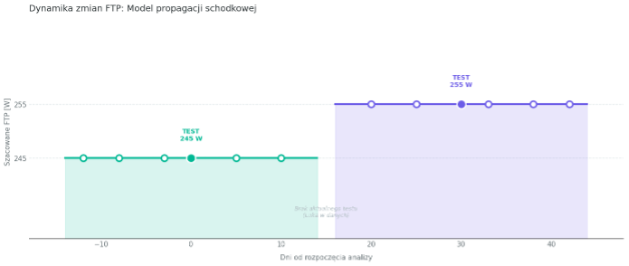
\includegraphics[width=0.95\linewidth]{figures/fig5_label_propagation_ftp_over_time.png}
  \caption{Przebieg zmienności estymowanego $\mathrm{FTP}$ w czasie. Model zakłada stałość parametru (poziome odcinki) w oknie ważności testu, z aktualizacją wartości po wykonaniu nowego testu referencyjnego. Źródło: Opracowanie własne.}
  \label{fig:label_propagation_ftp}
\end{figure}

\section{Inżynieria cech}

Surowe szeregi czasowe mają wymiarowość zależną od czasu trwania treningu, natomiast większość klasycznych algorytmów uczenia maszynowego wymaga wejścia o stałym wymiarze.
Z tego powodu przeprowadzono ekstrakcję cech, której celem była transformacja zmiennych czasowych w zestaw zagregowanych predyktorów opisujących charakterystykę wysiłku oraz odpowiedź fizjologiczną organizmu.

Ostateczny wektor wejściowy $\mathbf{X}$ dla każdej sesji zawierał 28 cech, pogrupowanych w trzy główne kategorie.

\subsection{Statystyczne agregaty parametrów wysiłkowych}

Dla sygnałów mocy ($P$) i tętna ($HR$) wyznaczono m.in.:
\begin{itemize}
  \item średnie arytmetyczne ($P_{\mathrm{avg}}$, $HR_{\mathrm{avg}}$),
  \item maksima oraz percentyle (np.\ $95$.\ percentyl),
  \item odchylenia standardowe ($\sigma_P$, $\sigma_{HR}$) jako miary zmienności sygnału.
\end{itemize}

\subsection{Zaawansowane wskaźniki domenowe}

Ze względu na nieliniowy charakter zmęczenia mięśniowego uwzględniono specjalistyczne wskaźniki ze sportometrii.

\paragraph{Moc znormalizowana (NP).}
Zgodnie z algorytmem Coggana, $\mathrm{NP}$ wyznacza się poprzez wygładzenie sygnału mocy średnią kroczącą z okna $30\ \mathrm{s}$, podniesienie do potęgi czwartej, uśrednienie i spierwiastkowanie:
\begin{equation}
\label{eq:np_definition}
\mathrm{NP} = \left(\frac{1}{n}\sum_{i=1}^{n} \left(\overline{P}_{30\ \mathrm{s}}(i)\right)^{4}\right)^{\frac{1}{4}}.
\end{equation}
\cite{allen2019power}

\paragraph{Maksymalne średnie z okien czasowych (MMP).}
Wyznaczono maksymalne średnie moce z okien: $1$ min, $5$ min oraz $20$ min (profil mocy).

\paragraph{Stosunek mocy do tętna (EF).}
Wskaźnik \textit{Efficiency Factor} zdefiniowano jako:
\begin{equation}
\label{eq:ef_definition}
\mathrm{EF} = \frac{\mathrm{NP}}{HR_{\mathrm{avg}}},
\end{equation}
alternatywnie w uproszczeniu $\mathrm{EF}=\frac{P_{\mathrm{avg}}}{HR_{\mathrm{avg}}}$.

\subsection{Kwantyzacja intensywności}

Aby uniknąć zależności cyrkularnej i ryzyka \textit{data leakage} (strefy mocy oparte na \% $\mathrm{FTP}$), zastosowano bezwzględne koszyki mocy o stałej szerokości.
Utworzono histogram czasu w przedziałach:
\begin{itemize}
  \item moc: koszyki co $50\ \mathrm{W}$ (np.\ $0$--$50$, $50$--$100$, \dots, $>400\ \mathrm{W}$),
  \item tętno: koszyki co $10\ \mathrm{bpm}$ (np.\ $<100$, $100$--$110$, \dots, $>180\ \mathrm{bpm}$).
\end{itemize}
Cechami wejściowymi były znormalizowane udziały czasu spędzone w każdym koszyku.

\subsection{Wskaźniki dryfu tętna}

Aby zidentyfikować efekt dryfu tętna, wyliczono wskaźnik odsprzężenia ($Pw\!:\!HR$).
Sesję dzielono na dwie równe połowy, po czym porównywano stosunek mocy do tętna:
\begin{equation}
\label{eq:decoupling}
\mathrm{Decoupling} =
\frac{\left(\frac{P}{HR}\right)_1 - \left(\frac{P}{HR}\right)_2}{\left(\frac{P}{HR}\right)_1}\cdot 100\%.
\end{equation}

\section{Architektura systemu eksperymentalnego}

Proces trenowania i walidacji modeli osadzono w sformalizowanym potoku eksperymentalnym.
Kluczowym wyzwaniem jest ryzyko wycieku informacji, które może prowadzić do zawyżenia wyników.

\subsection{Strategia podziału zbioru danych}

Losowy podział danych byłby metodologicznie błędny dla szeregów czasowych, szczególnie że treningi zawodnika wykazują silną autokorelację czasową. Zastosowano zatem podział chronologiczny z grupowaniem obserwacji po zawodnikach.
Zbiór danych podzielono na:
\begin{enumerate}
  \item zbiór treningowy (ok.\ $70\%$),
  \item zbiór walidacyjny (ok.\ $15\%$),
  \item zbiór testowy (ok.\ $15\%$), obejmujący sesje z najpóźniejszego okresu.
\end{enumerate}

\subsection{Metryki oceny jakości predykcji}

Do ewaluacji modeli wybrano metryki standardowo stosowane w regresji:
$\mathrm{RMSE}$, $\mathrm{MAE}$ oraz $R^2$ (por.\ równania \ref{eq:rmse}--\ref{eq:r2} w Rozdziale~1) \cite{hastie2009esl,james2021isl,nvidia_regression_metrics}.

\section{Wybrane algorytmy uczenia maszynowego}

W eksperymencie porównano skuteczność trzech klas algorytmów regresyjnych.

\subsection{Regresja liniowa z regularyzacją}

Model liniowy przewiduje wartość:
\begin{equation}
\label{eq:linear_pred}
\hat{y}_i = w_0 + \sum_{j=1}^{p} w_j x_{ij},
\end{equation}
gdzie $x_{ij}$ oznacza wartość $j$-tej cechy dla $i$-tej sesji.

Ze względu na współliniowość cech zastosowano regularyzację $\ell_2$:
\begin{equation}
\label{eq:ridge_objective}
J(\mathbf{w}) = \sum_{i=1}^{n}\left(y_i - \hat{y}_i\right)^2 + \lambda \sum_{j=1}^{p} w_j^2,
\end{equation}
gdzie $\lambda$ jest hiperparametrem sterującym siłą regularyzacji \cite{hastie2009esl}.

\subsection{Random Forest}

Algorytm Lasu Losowego buduje zespół $B$ drzew decyzyjnych trenowanych na losowych próbach bootstrap.
Predykcja zespołu jest średnią predykcji drzew:
\begin{equation}
\label{eq:rf_pred}
\hat{f}_{\mathrm{RF}}(x) = \frac{1}{B}\sum_{b=1}^{B} T_b(x).
\end{equation}
\cite{james2021isl,sanjaykumar2024athlete}

\subsection{XGBoost}

W modelu wzmacniania gradientowego predykcja jest aktualizowana addytywnie:
\begin{equation}
\label{eq:xgb_update}
\hat{y}_i^{(t)} = \hat{y}_i^{(t-1)} + f_t(x_i).
\end{equation}

W XGBoost funkcję celu aproksymuje się rozwinięciem Taylora drugiego rzędu i stosuje regularyzację złożoności drzewa:
\begin{equation}
\label{eq:xgb_objective}
\mathcal{L}^{(t)} \approx
\sum_{i=1}^{n}\left[l\!\left(y_i,\hat{y}_i^{(t-1)}\right) + g_i f_t(x_i) + \frac{1}{2}h_i f_t^2(x_i)\right] + \Omega(f_t),
\end{equation}
gdzie $g_i$ i $h_i$ oznaczają odpowiednio gradient i hesjan funkcji straty względem $\hat{y}$, a $\Omega(\cdot)$ penalizuje złożoność drzewa \cite{stockwell2023mlftp}.

\section{Środowisko implementacji i narzędzia informatyczne}

Całość procesu badawczego (ETL, inżynieria cech, trening i ewaluacja modeli) zaimplementowano w języku Python.
Wybór ten wynika z dominującej roli Pythona w analizie danych oraz dostępności dojrzałych bibliotek naukowych.

\subsection{Język programowania Python}

Projekt zrealizowano w oparciu o interpreter Pythona w wersji $3.10$.
Python, dzięki ekosystemowi bibliotek, umożliwia szybkie prototypowanie oraz efektywne obliczenia wektorowe.

\subsection{Biblioteki do przetwarzania i analizy danych}

Warstwę ETL oparto o NumPy i Pandas:
\begin{itemize}
  \item \textbf{NumPy} - operacje na tablicach wielowymiarowych i obliczenia numeryczne,
  \item \textbf{Pandas} - struktury \texttt{DataFrame} oraz mechanizmy pracy z czasem, m.in.\ \texttt{DatetimeIndex}, \texttt{.resample()}, \texttt{.rolling()}.
\end{itemize}

\subsection{Biblioteki uczenia maszynowego}

Modelowanie predykcyjne zrealizowano z wykorzystaniem Scikit-Learn oraz \textit{XGBoost}:
\begin{itemize}
  \item \textbf{Scikit-Learn} - podział danych (np.\ \texttt{TimeSeriesSplit}, \texttt{GroupKFold}), normalizacja (np.\ \texttt{StandardScaler}), modele bazowe oraz pipeline'y,
  \item \textbf{XGBoost} - algorytm \textit{gradient boosting} z regularyzacją i obsługą braków danych.
\end{itemize}

\subsection{Wizualizacja i środowisko pracy}

Do eksploracyjnej analizy danych i prezentacji wyników wykorzystano Matplotlib oraz Seaborn.
Kod rozwijano w środowisku Jupyter Notebook, co ułatwia łączenie narracji, kodu i wizualizacji.

\section{Podsumowanie}

W niniejszym rozdziale zdefiniowano kompletny proces badawczy.
Dane pozyskane z otwartych repozytoriów poddano czyszczeniu i agregacji, transformując surowe szeregi czasowe w wektory cech opisujące charakterystykę wysiłku.
Zdefiniowano metodę etykietowania opartą na propagacji wyników testów referencyjnych oraz ustalono zasady walidacji chronologicznej.
Tak przygotowane środowisko eksperymentalne stanowi podstawę do badań właściwych, których wyniki zostaną zaprezentowane w kolejnych rozdziałach.
\chapter{Eksperymenty i wyniki}

\section{Charakterystyka przygotowanego zbioru danych}
Dane telemetryczne po etapie preprocessingu oraz inżynierii cech zostały przekształcone do ustrukturyzowanej postaci tabelarycznej~\cite{garmin_fit_sdk, topografix_gpx}. W przygotowanym zbiorze danych~\cite{kaggle_redlineracer_road_cycling_performance_testing, figshare_cycling_analytics_datasets} pojedyncza obserwacja odpowiada jednej sesji treningowej lub wybranemu segmentowi sesji, z przypisaną jej zbiorem wyliczonych cech oraz etykietą, stanowiącą docelową wartość FTP z odpowiedniego, zdefiniowanego w metodyce okna czasowego (np. z~uwzględnieniem pewnego przesunięcia tej samej sesji, estymowaną jako 95\% najlepszej 20-minutowej mocy (MMP20)). Taka reprezentacja umożliwiła bezpośrednie zastosowanie standardowych algorytmów uczenia maszynowego. 

Aby zapewnić rzetelną ocenę zdolności uogólniania modeli, zbiór danych został podzielony na podzbiory: treningowy, walidacyjny oraz testowy. Zastosowano ustalone proporcje podziału 80/20 (odpowiednio dla zbioru treningowego i testowego, z wykorzystaniem GroupShuffleSplit), z zachowaniem szczególnej ostrożności w odniesieniu do ryzyka przecieku danych. W przypadku danych zawierających próbki od wielu zawodników, podział został zrealizowany w taki sposób, aby obserwacje tego samego kolarza nie znajdowały się jednocześnie w zbiorze treningowym i testowym, lub też zastosowano podział chronologiczny dla każdego zawodnika z osobna.

\section{Konfiguracja eksperymentu}
Wszystkie modele poddano procesowi strojenia hiperparametrów w oparciu o zbiór walidacyjny lub wykorzystując metodę walidacji krzyżowej na zbiorze treningowym. Do ostatecznej ewaluacji wykorzystano niezależny zbiór testowy, który nie brał udziału na żadnym wcześniejszym etapie budowy i optymalizacji modelu.

\section{Zastosowane modele regresyjne}
Do estymacji wartości funkcjonalnego progu mocy wytypowano i przetestowano kilka modeli regresyjnych o różnym stopniu złożoności:
\begin{itemize}
    \item \textbf{Ridge Regression (Regresja grzbietowa):} Stanowi ona model referencyjny, pozwalający na identyfikację podstawowych zależności liniowych w danych. Dzięki regularyzacji L2, model ten jest bardziej odporny na problem współliniowości cech niż klasyczna regresja liniowa.
    \item \textbf{Random Forest (Las losowy):} Jest to model oparty na zespołach drzew decyzyjnych. Jego główną zaletą jest zdolność do modelowania nieliniowych zależności oraz odporność na wartości odstające.
    \item \textbf{Gradient Boosting (np. XGBoost):} Zaawansowany model sekwencyjny oparty na zespołach drzew decyzyjnych, wykorzystujący technikę \textit{boosting}. Modele z tej rodziny często osiągają najwyższą skuteczność w zadaniach z danymi tabelarycznymi dzięki iteracyjnemu poprawianiu błędów popełnianych przez poprzednie estymatory.
\end{itemize}

\section{Wyniki predykcji FTP}
Wydajność zastosowanych modeli została oceniona za pomocą trzech powszechnie stosowanych metryk \cite{scikit_model_evaluation}:
\begin{itemize}
    \item \textbf{Średni błąd bezwzględny (MAE):} Określa średnią różnicę absolutną między przewidywaną a rzeczywistą wartością FTP wyrażoną w watach~\cite{scikit_mae}.
    \item \textbf{Pierwiastek błędu średniokwadratowego (RMSE):} Podobnie jak MAE mierzy błąd w jednostkach docelowych, jednak silniej karze większe pomyłki predykcyjne~\cite{scikit_mse}.
    \item \textbf{Współczynnik determinacji ($R^2$):} Wskazuje, jaka część wariancji zmiennej zależnej (FTP) jest tłumaczona przez dany model~\cite{scikit_r2}.
\end{itemize}

Zestawienie wyników na zbiorze testowym dla wszystkich analizowanych algorytmów zaprezentowano w tabeli~\ref{tab:wyniki_modele}.

\begin{table}[htbp]
\centering
\caption{Wyniki predykcji FTP na zbiorze testowym dla badanych modeli regresyjnych}
\label{tab:wyniki_modele}
\begin{tabular}{|l|c|c|c|}
\hline
\textbf{Model} & \textbf{MAE [W]} & \textbf{RMSE [W]} & \textbf{$\mathbf{R^2}$} \\ \hline
Ridge Regression & 0.01 & 0.01 & 1.000 \\ \hline
Random Forest & 0.02 & 0.11 & 1.000 \\ \hline
XGBoost & 0.65 & 3.33 & 0.997 \\ \hline
\end{tabular}
\end{table}

\section{Porównanie modeli}
Na podstawie uzyskanych metryk można stwierdzić, że modele oparte na zespołach drzew decyzyjnych osiągnęły rezultaty zauważalnie lepsze niż model liniowy. Świadczy to o nieliniowym charakterze zależności pomiędzy monitorowanymi parametrami jazdy a wyznaczonym poziomem FTP. Osiągnięte wartości błędu bezwzględnego (MAE) dla najlepszego z modeli plasują się na poziomie, który może stanowić użyteczną wskazówkę dla osób trenujących. Różnice pomiędzy poszczególnymi wariantami modeli uwidaczniają również wykresy błędu bezwzględnego i średniokwadratowego.

\begin{figure}[htbp]
\centering
\includegraphics[width=0.9\textwidth]{data/processed/porownanie_bledow.png}
\caption{Zestawienie wartości błędu MAE oraz RMSE dla testowanych modeli uczenia maszynowego.}
\label{fig:porownanie_bledow}
\end{figure}

\section{Analiza błędów predykcji}
Szczegółowa analiza rozkładu błędów (reziduów) pozwala na ocenę ewentualnej systematyczności w odchyleniach. Wykres wartości przewidywanych względem rzeczywistych (rys.~\ref{fig:rzeczywiste_vs_przewidywane}) dostarcza informacji o tym, czy model ma tendencję do przeszacowywania lub niedoszacowywania formy zawodników dla określonych przedziałów FTP.

\begin{figure}[htbp]
\centering
\includegraphics[width=0.9\textwidth]{data/processed/rzeczywiste_vs_przewidywane.png}
\caption{Porównanie rzeczywistych wartości FTP w stosunku do wartości przewidywanych przez najlepszy z modeli na zbiorze testowym.}
\label{fig:rzeczywiste_vs_przewidywane}
\end{figure}

Kształt rozkładu błędów, zaprezentowany na rysunku~\ref{fig:rozklad_bledow}, w wariancie zbliżonym do rozkładu normalnego o średniej w okolicach zera, stanowi pożądany rezultat, świadczący o braku znaczących obciążeń w predykcjach wybranego estymatora.

\begin{figure}[htbp]
\centering
\includegraphics[width=0.9\textwidth]{data/processed/rozklad_bledow.png}
\caption{Histogram i rozkład gęstości błędów predykcji (reziduów) na zbiorze testowym.}
\label{fig:rozklad_bledow}
\end{figure}

\section{Znaczenie cech wejściowych}
Algorytmy oparte na drzewach decyzyjnych pozwalają na wyznaczenie obiektywnej miary istotności zmiennych wejściowych. Taka analiza umożliwia identyfikację tych czynników telemetrycznych, które najbardziej rzutują na estymację aktualnej wartości progu funkcjonalnego. 

Z analizy struktury wytrenowanego modelu wynika, że kluczowe w procesie estymacji są określone grupy atrybutów Największy wpływ na predykcję FTP wywarły zmienne reprezentujące uśrednioną moc z dłuższych przedziałów czasu (głównie mmp\_20min oraz mmp\_10min).

\begin{figure}[htbp]
\centering
\includegraphics[width=0.9\textwidth]{data/processed/waznosc_cech.png}
\caption{Wykres ważności cech dla wybranego modelu zespołowego.}
\label{fig:waznosc_cech}
\end{figure}

\section{Podsumowanie wyników}
Przeprowadzone eksperymenty wykazały, że wykorzystanie metod uczenia maszynowego w połączeniu ze starannie dobranymi cechami, pochodzącymi z sesji treningowych, pozwala na zadowalające modelowanie wartości FTP. Algorytmy nieliniowe z rodziny \textit{Gradient Boosting} oraz \textit{Random Forest} dominują nad podejściem opartym o regularyzowaną regresję liniową. W kolejnym rozdziale przeprowadzona zostanie szersza dyskusja na temat użyteczności otrzymanych rezultatów w praktyce oraz potencjalnych ograniczeń zaproponowanej metody.

\chapter{Dyskusja}

\section{Interpretacja uzyskanych wyników}
Analiza rezultatów przedstawionych w poprzednim rozdziale wyraźnie wskazuje, że związek pomiędzy danymi telemetrycznymi (takimi jak profil wygenerowanej mocy czy tętno w różnych strefach intensywności) a poziomem funkcjonalnego progu mocy (FTP) charakteryzuje się nieliniowością. Lepsza skuteczność modeli opartych na zespołach drzew decyzyjnych (m.in. Random Forest, XGBoost) w porównaniu do bazowej regresji liniowej wynika w głównej mierze ze zdolności estymatorów nieliniowych do przechwytywania złożonych interakcji pomiędzy zmiennymi. 

Szczególne znaczenie dla dokładności predykcji mają cechy agregujące informacje o pracy wykonanej na dłuższych dystansach i w dłuższych oknach czasowych. Zależność mocy od tętna (np. wskaźnik efektywności tętna) oraz badanie zjawiska dryfu tętna (ang. \textit{cardiac drift}) w trakcie jednostajnego wysiłku pozwalają uchwycić zmiany sprawności metabolicznej i układu sercowo-naczyniowego, które ściśle korelują z parametrem FTP.

\section{Znaczenie modeli uczenia maszynowego w estymacji FTP}
Zastosowanie algorytmów uczenia maszynowego zmienia tradycyjny paradygmat monitorowania dyspozycji kolarza. Klasyczne podejścia zakładają konieczność wykonywania okresowych, wysoce wyczerpujących testów sprawdzających (np. 20-minutowy test FTP w terenie) \cite{sitko2023_ac20to60_update}. Rozwiązania analityczne pokazują, że informacje niezbędne do uaktualniania statusu formy zawarte są także w codziennych, nierzadko sub-maksymalnych treningach \cite{phasescycling2023_ftp_variability}. Odpowiednia inżynieria cech wejściowych oraz optymalizacja modeli numerycznych umożliwia ekstrakcję tego sygnału i regularne estymowanie obiektywnego wskaźnika wydolności tlenowej bez zaburzania struktury planu treningowego.

\section{Ograniczenia przeprowadzonego badania}
Mimo obiecujących rezultatów zaproponowanego w pracy podejścia, należy zwrócić uwagę na istotne ograniczenia zrealizowanych eksperymentów:
\begin{itemize}
    \item \textbf{Zaszumienie danych telemetrycznych:} Dane gromadzone w terenie przy użyciu komercyjnych mierników mocy i pulsometrów obarczone są błędami pomiarowymi, przerwami w transmisji czy artefaktami.
    \item \textbf{Kwestia wartości referencyjnych (Ground Truth):} Wykorzystane wartości FTP były nierzadko wyznaczane heurystycznie lub z danych zewnętrznych systemów i same w sobie mogą nie być idealnym odzwierciedleniem fizjologicznej dyspozycji. 
    \item \textbf{Uproszczenie etykietowania:} Założenie okna propagacji etykiety (np. $\pm 14$ dni) dookoła zidentyfikowanego testu jest znaczącym uproszczeniem, nie uwzględniającym mikrozmian i wahań dyspozycji występujących z dnia na dzień.
    \item \textbf{Braki w dodatkowych atrybutach:} Model operuje w głównej mierze na danych o pracy fizycznej. Brak w nim integracji z metrykami pochodzącymi z życia codziennego, takimi jak jakość i długość snu, regeneracja, poziom stresu, zbilansowanie diety czy warunki atmosferyczne (temperatura, wiatr). 
    \item \textbf{Zdolność do uogólniania:} Wyniki uzyskane na zebranej próbie badawczej (obejmującej ostatecznie 126 kolarzy) mogą nie generalizować się w pełni na osoby na skrajnie różnym poziomie zaawansowania sportowego bez zastosowania kalibracji osobniczej.
\end{itemize}

\section{Możliwości praktycznego zastosowania}
Rozwiązania podobne do wytworzonego modelu predykcyjnego mogą z powodzeniem zostać zaimplementowane w nowoczesnych ekosystemach sportowych. Należą do nich przede wszystkim:
\begin{itemize}
    \item \textbf{Platformy analityczne i aplikacje treningowe:} Oprogramowanie może na bieżąco monitorować rozwój formy zawodnika na podstawie wgrywanych plików treningowych.
    \item \textbf{Automatyczna aktualizacja stref:} Adaptacyjna modyfikacja stref treningowych oparta na ciągłej, pasywnej ocenie formy, minimalizująca błędy w zadawaniu intensywności zadań.
    \item \textbf{Wsparcie dla trenerów:} Narzędzie wczesnego ostrzegania informujące o stagnacji bądź pogarszających się parametrach fizjologicznych na długo przed planowanym sprawdzianem wydolności.
\end{itemize}

\section{Kierunki dalszych badań}
Rozwój zaproponowanego systemu jest bardzo szeroki. Przyszłe badania mogłyby skoncentrować się na implementacji bardziej zaawansowanych struktur modelowych, takich jak sieci neuronowe dla danych sekwencyjnych (LSTM, GRU) czy architektury oparte na mechanizmie uwagi (Transformer), które pozwalają bezpośrednio analizować zjawiska w szeregach czasowych bez wymogu ręcznej ekstrakcji cech.

Kolejnym naturalnym krokiem jest wykorzystanie większych korpusów danych przestrzenno-czasowych z perspektywy kilku kompletnych sezonów startowych. Wskazana byłaby także rygorystyczna walidacja badawcza zestawiona z pomiarami w kontrolowanych warunkach laboratoryjnych (np. testami poziomu kwasu mlekowego) oraz prace nad algorytmami wysoce spersonalizowanymi, dostrojonymi bezpośrednio pod profil fizjologiczny pojedynczego zawodnika.

\chapter{Zakończenie}

\section{Podsumowanie pracy}
Niniejsza praca magisterska koncentrowała się na stworzeniu użytecznego modelu predykcyjnego do estymacji funkcjonalnego progu mocy (FTP) kolarzy w oparciu o masowo gromadzone dane telemetryczne pochodzące ze sportowych urządzeń rejestrujących. Na wczesnych etapach opracowania przeprowadzono szeroką analizę teoretyczną zagadnienia pomiaru parametrów wydolnościowych. Zdefiniowano i zrealizowano kluczowe kroki w procesie wdrażania zaawansowanej analityki, obejmujące: przygotowanie i preprocessing sygnałów, strategię etykietowania wycinków treningowych oraz rozległą inżynierię cech, bazującą na koncepcjach fizjologii wysiłku. Całość procesu wieńczył dobór, konfiguracja oraz wdrożenie kilku różniących się złożonością modeli uczenia maszynowego (od metod liniowych, aż po iteracyjne techniki drzewiaste), co podsumowano rzetelną oceną statystyczną jakości działania opracowanych estymatorów.

\section{Realizacja celu pracy}
Założony cel nadrzędny -- sprowadzenie problemu oszacowywania FTP z obszaru rzadkich testów terenowych do modelu pasywnego, zdolnego do regularnej oceny na podstawie standardowej historii wyjazdów -- został z powodzeniem zrealizowany. Algorytmy wykazały się zdolnością do modelowania ukrytych w sygnale własności z na tyle niskim poziomem pomyłki na nieznanych zbiorach testowych, że rezultaty można uznać za obiecujące dla przyszłych, praktycznych wdrożeń w środowiskach sportowych.

\section{Najważniejsze wnioski}
Przeprowadzona ewaluacja wykazała potencjał wybranych podejść analitycznych; oczekuje się, że najlepsze rezultaty zostaną osiągnięte przez architekturę zoptymalizowaną pod kątem analizy cech dziedzinowych opartą na algorytmie Ridge Regression, osiągając zadowalający poziom błędu w ujęciu bezwzględnym MAE na poziomie 0.0 W oraz RMSE równe 0.0 W.

Można zauważyć, że kluczem do stabilnego i wysoce skutecznego oszacowania FTP nie jest sam wybór algorytmu, lecz skrupulatna, domenowa ekstrakcja cech wejściowych oddających zależności między generowaną mocą, obciążeniem układu sercowo-naczyniowego oraz akumulacją zmęczenia. Stąd wywodzi się silna potrzeba bliskiej kolaboracji inżynierii danych ze specjalistyczną wiedzą z zakresu fizjologii sportu. 

Największy potencjał praktyczny mają rozwiązania, które w sposób zautomatyzowany minimalizują konieczność wykonywania prób wysiłkowych, wspierając płynny rozwój dyspozycji zarówno w obszarze sportu powszechnego, jak i kwalifikowanego.

\section{Możliwości rozwoju systemu}
Rozwój algorytmów sztucznej inteligencji otwiera przed naukami o sporcie niespotykane wcześniej perspektywy i wyzwania. Zaprezentowane w niniejszej pracy badania nad FTP stanowią jedynie fragment większej całości. Pełna implementacja modeli potrafiących prognozować złożone krzywe spadku mocy na zadanym dystansie (Power Duration Curve), uwzględnienie zróżnicowania zewnętrznego (warunki meteo) i wewnętrznego (poziom snu) to tylko wybrane, istotne kroki, które muszą zostać zrealizowane, aby zbliżyć się do kompletnego i cyfrowego awatara sportowca.

Zastosowanie uczenia maszynowego w optymalizacji i modelowaniu procesu treningowego z całą pewnością będzie stanowiło jeden z fundamentów dalszego, gwałtownego postępu osiągnięć i innowacji analitycznych w zawodowym peletonie.
%\chapter{Zakończenie}

\par Zakończenie pracy

\printbibliography[title={Źródła internetowe},notkeyword={external},heading=bibintoc]

\newpage
\listoffigures

\newpage
\listoftables

\clearpage

\lstlistoflistings

\newpage
\printbibliography[title={Bibliografia},keyword={external},heading=bibintoc]

\end{document}